\documentclass{beamer}

%\usepackage{beamerthemesplit} %Activate for custom appearance
\usetheme{Hannover}
\usecolortheme{rose}

%Unnumbered footnotes
\newcommand\ufoot[1]{
\begingroup
\renewcommand\thefootnote{}\footnote{#1}
\addtocounter{footnote}{-1}
\endgroup
}



\title{Intro to Git\\Part I}
\subtitle{IB 516 Analytical Workflows}
\author{}
\date{}

\begin{document}

\frame{\titlepage}

\section[Outline]{}
\frame{\tableofcontents}

\section{Introduction to version control with Git}

\frame{
	\frametitle{What is a version control system?}

	\begin{itemize}
	\item Records changes in a set of files over time so that you can recall specific versions later.
	\item Allows 'time travel' back and forth from any previous time in your project development.
	\item Allows 'peaceful coexistence and exchange of info between 'parallel universes' of a project'
	\item Allows stable and efficient collaborations (with others and with your past self) that produce reproducible work.
	\end{itemize}
	
}


\frame{
	\frametitle{In practice}
	
	\begin{itemize}
			\item Avoid appending version/date to filenames.
			\item Compare changes over time.
			\item Revert the entire project back to a previous state.
			\item View or revert selected files back to a previous state.
			\item See who last modified something that might be causing a problem, 
			who introduced the bug and when, and more. 
			\item If you screw things up or lose files, you can easily recover. 
			\item You get all this for very little effort / overhead (aside from startup 
			costs for learning).
	\end{itemize}
	
	\ufoot{\tiny{https://git-scm.com/book/en/v2/Getting-Started-About-Version-Control}}

}


\frame{
	\frametitle{Visualizing a version controlled project through time}
	
	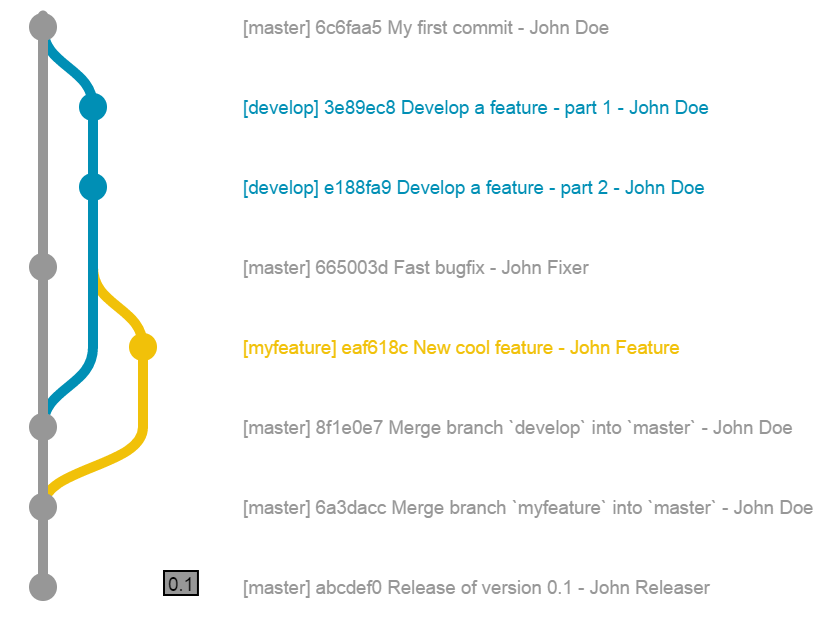
\includegraphics[scale = 0.3]{figs/pretty_branch_graph}
	
	\ufoot{\tiny{https://stackoverflow.com/a/24107223}}


}

\frame{
	\frametitle{Version control in Git:\\How Git stores data}
	
	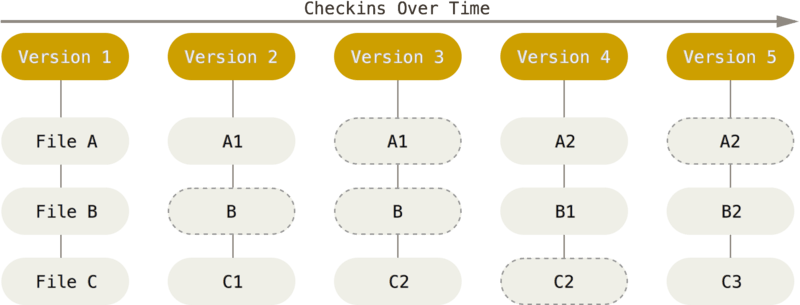
\includegraphics[scale = 0.3]{figs/how_git_stores_data}
	
	\ufoot{\tiny{http://git-scm.com/book/en/v2/Getting-Started-What-is-Git}}
	
	
}




\section{Basic Workflow}


\frame{
	\frametitle{A file's lifecyle}
	
	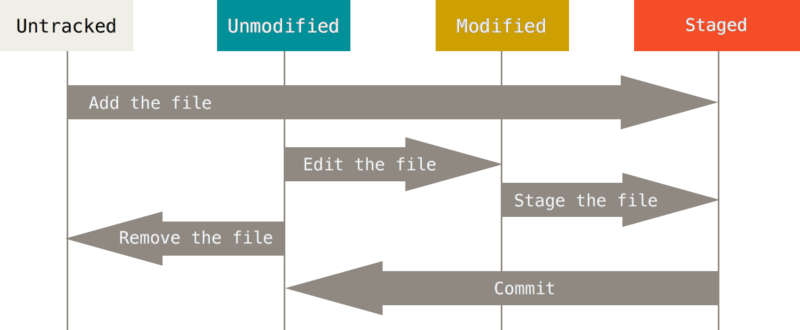
\includegraphics[scale = 0.3]{figs/lifecycle}
		
	\ufoot{\tiny{http://git-scm.com/book/en/v2/Getting-Started-What-is-Git}}
	
	\tiny{*We haven't talked about $staging$ which is an intermediate step between modifying a file and committing it. Git allows you to choose which modified files will be $staged$ (i.e. flagged for inclusion) as part of the next commit. Typically we will want to commit all modifications. Github Desktop automatically stages all modifications, so we don't need to think too much about staging at the moment.}
	
}

\frame{
	\frametitle{Git jargon}
	
	\centering
	repository -- staging -- commit \\
	local -- remote \\
	pull -- fetch -- push \\
	master (main) -- branch (feature branch) -- merge \\
	origin -- clone -- fork

}
	
\frame{
	\frametitle{Commit messages}
	
	\begin{itemize}
		\item Use the `imperative mood.' %(e.g. ``finish your homework'')
        		\item Complete the sentence: \\
        		 \emph{ ``If this commit is adopted , it will...''}
       		\item Capitalize the first word.
		\item Do not use a period.
	\end{itemize}
	
	\centering
	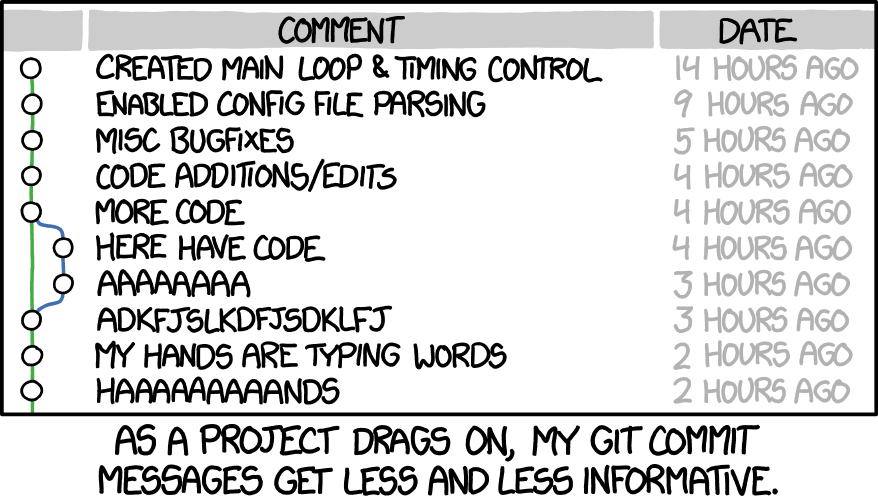
\includegraphics[scale = 0.5]{figs/commit_messages} \\
	
	\ufoot{\tiny{https://chris.beams.io/posts/git-commit/}}
}


\end{document}
